\documentclass[11pt, oneside]{article} 
\usepackage{geometry}
\geometry{letterpaper} 
\usepackage{graphicx}
	
\usepackage{amssymb}
\usepackage{amsmath}
\usepackage{parskip}
\usepackage{color}
\usepackage{hyperref}

\graphicspath{{/Users/telliott/Github/calculus_book/png/}}
% \begin{center} 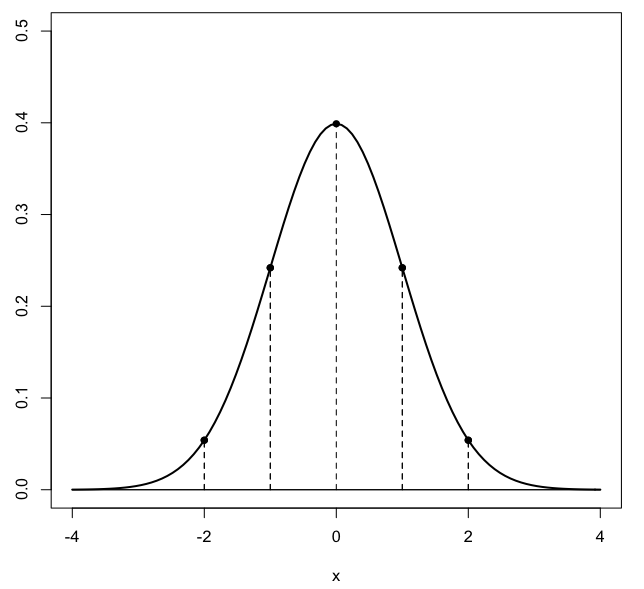
\includegraphics [scale=0.4] {gauss3.png} \end{center}

\title{More induction}
\date{}

\begin{document}
\maketitle
\Large

Previously, we showed that the sum of integers
\[ \sum_{k=1}^{k=n} = \frac{1}{2} \cdot n(n+1) \]

and presented this "proof without words":

\begin{center} 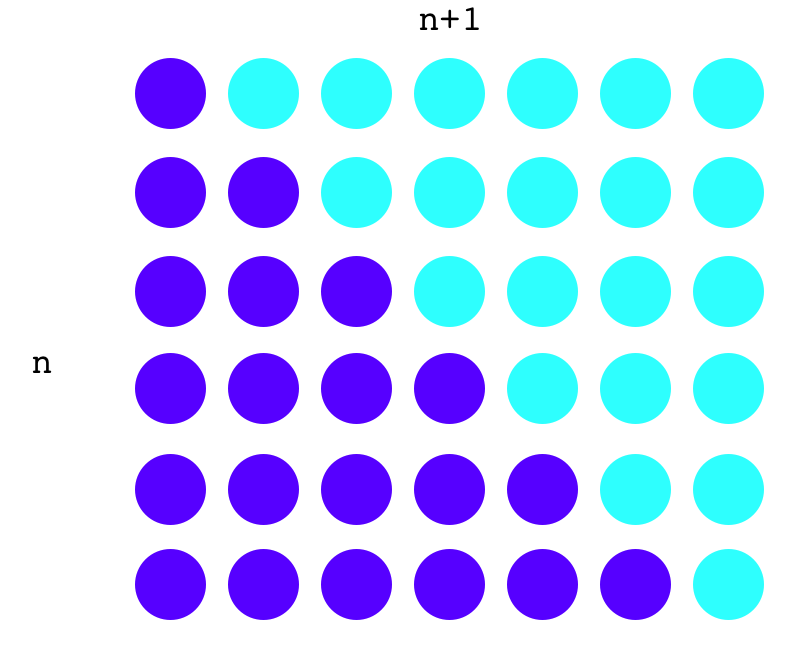
\includegraphics [scale=0.25] {sum_n.png}\end{center}

\subsection*{Derivation using sums}
It seems a shame to spoil such a beautiful proof as the one above,  let alone the inductive proof,  by saying anything more, but I can't resist.  

You will notice that we were given the formula and only proved it true.  As we quoted Archimedes in the first chapter

\begin{quote}it is of course easier, when we have previously acquired by the method some knowledge of questions, to supply the proof than it is to find the proof without any previous knowledge.\end{quote}

I'd like to derive the equation we have been using using algebra.  The general method can be used to get the sum of the squares of integers, or their cubes, or even higher powers.

For any number $k$ it is true that
\[ (k+1)^2 = k^2 + 2k + 1 \]
So consider what happens if we sum the values from $k=1 \rightarrow n$ for each of these terms
\[ \sum_{k=1}^n (k+1)^2 = \sum_{k=1}^n k^2 + \sum_{k=1}^n 2k + \sum_{k=1}^n 1 \]

If the equation is valid for any individual $k$, then it is also true adding the equations for all $k$ from $1$ up to $n$.

Rearranging
\[ \sum_{k=1}^n (k+1)^2 - \sum_{k=1}^n k^2 = \sum_{k=1}^n 2k + \sum_{k=1}^n 1 \]
Now think about the left-hand side in our equation. 
\[ \sum_{k=1}^n (k+1)^2 - \sum_{k=1}^n k^2 \]
If we count down rather than up, start with $k=n$.  We have the following terms
\[ k = n \ \ \text{gives} \ \ (n+1)^2 - (n)^2 \]
\[ k = n-1 \ \ \text{gives} \ \ (n)^2 - (n-1)^2 \]
\[ k = n-2 \ \ \text{gives} \ \  (n-1)^2 - (n-2)^2 \]
\[ \cdots \]
\[ k = 1 \rightarrow \ \ (2)^2 - (1)^2 \]

We must add all of these together.  But notice how all the terms except the first and last cancel.  For example we have $-(n)^2$ in the top line and $(n)^2$ in the second. This is called a "collapsing" or "telescoping" sum.  We obtain
\[ S = (n+1)^2 - 1 \]\

Bringing back the right-hand side  we have
\[ (n+1)^2 - 1 = \sum_{k=1}^n 2k + \sum_{k=1}^n 1 \]

We can bring the constant factor $2$ out of the sum, and also, we recognize that the sum of the value $1$ a total of $n$ times is just $n$.
\[ (n+1)^2 - 1 = 2\sum_{k=1}^n k + n \]

Subtract $n$ from both sides.  The left hand side is
\[ (n+1)^2 - 1 - n = n^2 + n = n(n+1) \]
Finally, divide by $2$:
\[ \sum_{k=1}^n k = \frac{n (n+1)}{2} \]
That's our formula.

\subsection*{sum of integer squares}
\begin{center} 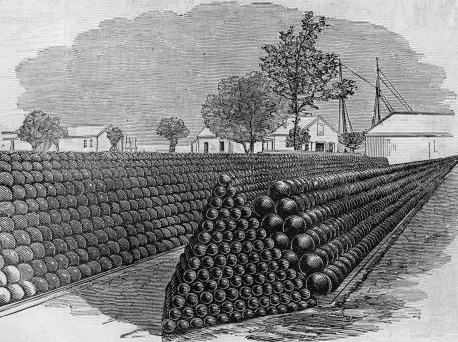
\includegraphics [scale=0.4] {cannonballs.png} \end{center}

Have you ever seen a square stack of marbles, or cannonballs?  The number of elements on each level is the square of a natural number.  We ask, what is the total number:
\[ S = 1^2 + 2^2 + \dots + n^2 = \ ? \]

The answer is not so obvious:
\[ S = \frac{1}{3} \cdot n \cdot (n + \frac{1}{2}) \cdot (n + 1) \]
although, given the formula for the volume of a cone or pyramid, the factor $1/3$ is not surprising.

It is often given as
\[ S = \frac{n(n+1)(2n+1)}{6} \]
The base case is correct:  $1(2)(3)/6 = 1$.

Here is the inductive proof.  

Add the square of $n+1$ to both sides:
\[ S + (n+1)^2 = \frac{n(n+1)(2n+1)}{6} + (n+1)^2 \]
\[ = \frac{n(n+1)(2n+1) + 6(n+1)^2}{6} \]
Factor $(n+1)$ in the numerator
\[ = \frac{(n+1) \ [ \ n(2n+1) + 6(n+1)}{6} \]

I always find the algebra tricky for this part.  Recognize that the rest of the numerator is:
\[ = 2n^2 + 7n + 6 \]
\[ = (n + 2)(2n + 3) \]
\[ = [ \ (n+1) + 1 \ ] \cdot [ \ (2(n+1) + 1 \ ]  \]
Putting it all together:
\[  S = \frac{(n+1) \cdot [ \ (n+1) + 1 \ ] \ \cdot \ [ \ 2(n+1) + 1 \ ]  \ ]}{6} \]
which is exactly the same as the formula first given, substituting $n+1$ for $n$.

\subsection*{Fibonacci example}

The Fibonacci numbers (or \emph{sequence}) start(s) with
\[ 1, 1 \]
The third number is the sum of the previous two
\[ 1, 1, 2 \]
and the general formula is that
\[ F_n = F_{n-2} + F_{n-1} \]
The first ten numbers are
\[ 1, 1, 2, 3, 5, 8, 13, 21, 34 \dots \]

We will use induction to prove that the sum of the first $n$ Fibonacci numbers is
\[ 1 + 1 + 2 + \dots + F_n = F_{n+2} - 1 \]
We assume that the formula is correct for $F_{n - 1}$:
\[ 1 + 1 + 2 + \dots + F_{n-1} = F_{n+1} - 1 \]
Add $F_{n}$ to both sides
\[ 1 + 1 + 2 + \dots + F_{n} = F_{n} + F_{n+1} - 1 \]
\[ = F_{n+2} - 1 \]

This completes the induction.

The base case is 
\[ 1 + 1 = 2 - 1 \]

$\square$

Another way to check this is to write the sum as

\begin{verbatim}
 1 + 1 + 2 + 3 + 5 + 8 + ..      .. + F_{n}   + F_{n+1}
     1 + 1 + 2 + 3 + 5 + 8 + ..  .. + F_{n-1} + F_{n}
 -------------------------------------------------------
 1 + 0 + 1 + 1 + 2 + 3 + ..      .. + F_{n-2} + F_{n-1}
\end{verbatim}

Subtracting the second sum from the first, we obtain the third:
\[ \sum F_{n+1} - \sum F_n =  \sum F_{n-1} + 1  \]
\[ F_{n+1}  =  \sum F_{n-1} + 1  \]
which rearranges to give the formula.

\subsection*{example}

A last example has an inequality.  For positive integer $n$:
\[ \sum \frac{1}{n^2} \le 2 - \frac{1}{n} \]

If $n=1$ we have equality $1 = 2 - 1$; for $n=2$ we have $1 + 1/4 < 3/2$.  For $n = 3$, we have that $1 + 1/2 + 1/9 < 2 - 1/9$ so we suppose that (excepting $n=1$):

\[ \sum \frac{1}{n^2} < 2 - \frac{1}{n} \]
In fact, this seems to get better as $n$ increases.  Here is an inductive proof.

Assume the formula is true for $n$.  Then for $n+1$ we will have:
\[ \sum \frac{1}{(n+1)^2} < 2 - \frac{1}{n} + \frac{1}{(n+1)^2}  \]

Observe first that
\[ \frac{n}{n + 1} < 1; \ \ \ \  \frac{n(n+1)}{(n + 1)^2} < 1 \]

So the new term on the right hand side obeys this relationship:
\[ \frac{1}{(n + 1)^2} <  \frac{1}{n(n+1)} = \frac{1}{n} - \frac{1}{n + 1} \]
and we just substitute:
\[ \sum \frac{1}{(n+1)^2} < 2 - \frac{1}{n} + \frac{1}{n} - \frac{1}{n + 1} \]
\[ \sum \frac{1}{(n+1)^2} < 2 - \frac{1}{n + 1} \]

$\square$


\end{document}  